\newcommand{\Harmonization}{
  \begin{figure}
    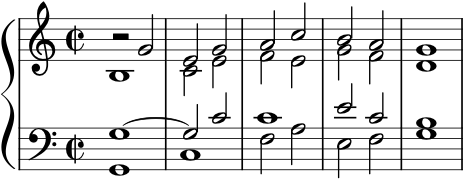
\includegraphics[width=5.5cm]{fig/piston.png}
    \hspace{1cm}
    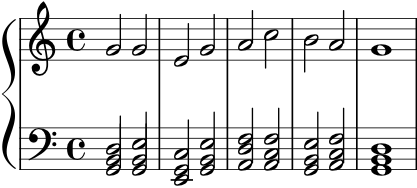
\includegraphics[width=5cm]{fig/fharm.png} \\
    \begin{flushleft}
    \begin{small}
     \hspace{2.35cm} V \ \ \ \ \ \ \ \,I \ \ \ \ \ \ \ \,IV \,VI \ \,III \ IV \ \ \,V
     \hspace{2.6cm} V \ \ \ \ \ \ \ \,I \ \ \ \ \ \,IV VI \,III\,IV \ \ V
    \end{small}
    \end{flushleft}
    \caption{Harmonization by Piston (left) and \fharm (right)}
    \Description{Harmonization by Piston (left) and \fharm (right)}
    \label{fig:harmonization}
  \end{figure}
}

\newcommand{\HarmonizationMT}{
  \begin{figure}
    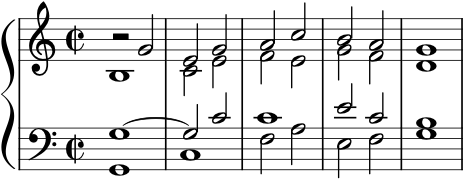
\includegraphics[width=5.5cm]{fig/piston.png}
    \hspace{1cm}
    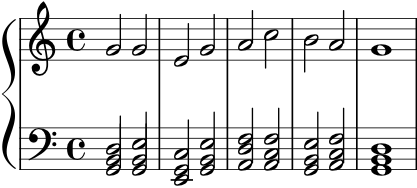
\includegraphics[width=5cm]{fig/fharm.png} \\
    \begin{flushleft}
    \begin{small}
     \hspace{2.35cm} V \ \ \ \ \ \ \ \,I \ \ \ \ \ \ \ \,IV \,VI \ \,III \ IV \ \ \,V
     \hspace{2.6cm} V \ \ \ \ \ \ \ \,I \ \ \ \ \ \,IV VI \,III\,IV \ \ V
    \end{small}
    \end{flushleft}
    \caption{Harmonization by Music Tools (to be replaced by real figure)}
    \Description{Harmonization by Music Tools}
    \label{fig:harmonizationMT}
  \end{figure}
}

\section{Harmony}
\label{sec:harmony}

Harmony refers to simultaneously sounding tones (chords) and its study
is primarily concerned with the progression of chords throughout a
piece of music. It is in essence the of dual of counterpoint. In this
section we formalize a small part of the classic text
\citet{piston-harmony}, in particular part of Chapter~9 which is
concerned with techniques for harmonizing a given melody.

\subsection{Harmonic Progression}
\label{sec:harmony:prog}

The primary Example~9.1 in Piston's text
(Figure~\ref{fig:harmonization} left) shows a
sample four part SATB harmonization in C~major. The melody is the
series of highest notes, i.e., the soprano (S) line, while the other three
parts alto (A), tenor (T), and bass (B) are the melodies below
it. Roman numerals denote the names of the triads at each vertical
slice. Note that even though there are four voices there are only
three distinct pitches sounding at each vertical slice (where tones an
octave apart are considered to have the same relative pitch). As is
typical the root of the triad is always doubled. Also note that all
triads are in root position (meaning the root is in the bass voice),
as Piston restricts to this case initially in the chapter (he does
relax it later). The goal of a harmonization is both to create an
aesthetically pleasing chord progression as well as fluid melodies in
each voice (called voice leading) and independence of each music
line (in other words good counterpoint). In this chapter
Piston gives advice on how to achieve these goals.

\Harmonization

We would like to formalize some of this advice and apply it to
automate harmonization of melodies. We start with selection of the
sequence of triads, in other words the harmonic progression. Earlier
in the text (on page~23) Piston presents a Table of Usual Root
Progressions, noting which triads usually follow a given one and
which are sometimes used or rare. It is easy to encode this in Agda
using the \texttt{Triad} datatype from Section~\ref{sec:music}.

\begin{alltt}
record NextTriad : Set where
  constructor nextTriadb
  field
    usual : List Triad; sometimes : List Triad; rare : List Triad

rootProgression : Triad \(\rightarrow\) NextTriad
rootProgression I   = nextTriad (IV :: V :: []) (VI :: []) (II :: III :: [])
rootProgression II  = nextTriad (V :: []) (IV  :: VI :: []) (I :: III :: [])
-- other cases omitted for space
\end{alltt}

It is easiest to create a harmonic progression in reverse, to
ensure that one ends a musical phrase with either a full (V--I) or half (V)
cadence, and work backward from there. So we would like to invert this
table to give a list of likely triads to precede a given triad. This
would normally be straightfoward but here we see a disadvantage of
using Agda. As is typical with languages based on dependent type
theories, equality is a very subtle concept and even determing if a
term is a member of a list is nontrivial.

In Haskell this would be easy---there is an \texttt{Eq} typeclass and a
method for automatically generating equalities. In the Agda Standard
Library~\citep{agda-stdlib} is a relation with a constructive proof of
membership, and requires far more effort than we need. Alternatives
include defining decidable equality for triads (which requires writing
out 49 cases) or mapping to natural numbers and using already
implemented decidable or boolean equality for those. For now we simply
write the inverse function manually, excluding the rare cases.

\begin{alltt}
previousTriads : Triad → List Triad
previousTriads I   = V :: IV :: VII :: []
previousTriads II  = VI :: IV :: []
-- other cases omitted for space
\end{alltt}

\subsection{Completing the Harmonization}
\label{sec:harmony:complete}

As Piston does we require the harmonizing triad to include the melody
note. We use a function \texttt{harmonizations} to generate a list of
all candidate harmonizations for a given melody. For space
considerations we refer the reader to the supplement
\texttt{Harmony.agda} for its definition. Here again we encounter difficulties
with equality and membership. We use a bit vector to represent the
set of scale degrees in a triad, where each scale degree is mapped to
an element of \texttt{Fin 7}.

We next restrict to progressions ending in a half cadence (V) to match
Piston's example. This results in 25 candidate progressions.

See Figure~\ref{fig:harmonizationMT}, which is currently just a copy of
the other figure, but included here now for space.

\HarmonizationMT

\subsection{Comparison with Previous Work}
\label{sec:harmony:compare}

Most of the Haskell-based
work~\citep{magalhaes-harmtrace,koops-fharm,magalhaes-fcomp} has
focused on harmony. In particular \fharm~\citep{koops-fharm} tackles
the problem of harmonization of a melody;
Figure~\ref{fig:harmonization} right shows their harmonization of
Piston's example. Their method is quite different from
ours. Instead of using Piston's table of root progressions they use a
more sophisticated hierarchical grammar from previous
work~\citep{magalhaes-harmtrace}.
More specifically, they first require the melody notes to be members of
the harmonizing chords, then use their previous work to try to create
a harmonic analysis of every possible sequence of chords that arises,
choosing the one that most closely fits their grammar.

Although the result produced by \fharm is not bad, it clearly leaves
room for improvement. Noted in
the paper is that no attention is given to voicing (how each of the
four parts flows horizontally and how the lines interact---in other
words the counterpoint). They use inversions (in which the
third or fifth of the chord is in the bass) to ensure each melody line
does not move too much, but as the harmonizing triads are all in close
postion separated from the melody, the result sounds like a soprano
melody with block chord accompaniment, rather than four independent
lines.

Furthermore, \fharm always double the melody note, not the root note
as Piston does (and as preferred in four-part harmony in general).
Also, minimizing the number of parse errors as a means
to choose the best harmonization does not necessarily have a musical
meaning.

TODO: More comparison.
